\documentclass[12pt,letterpaper]{article}
\usepackage{graphicx} % For including figures
\usepackage{amsmath,amssymb,amsfonts}
\usepackage{physics}
\usepackage[utf8]{inputenc}
\usepackage[T1]{fontenc}
\usepackage[english]{babel}
\usepackage{geometry}
\usepackage{xcolor}
\usepackage{mathtools}
\usepackage{bm}
\usepackage{float} % For better figure placement with [H]
\usepackage{caption} % For better caption formatting
\usepackage{subcaption} % For subfigures
\usepackage{microtype} % For better typography and margin justification

\geometry{margin=1in}
\definecolor{crystal}{RGB}{30, 100, 180}
\raggedbottom

% Caption setup for better line breaks
\captionsetup{width=0.9\textwidth}
\captionsetup[subfigure]{width=0.95\textwidth}

% Configure hyperlinks
% Load hyperref and bookmark packages after all other packages
\usepackage[
    pdfencoding=unicode,
    breaklinks=true,
    hidelinks,
    pdfusetitle,
    pdfdisplaydoctitle=true,
    pdfstartview=FitH,
    colorlinks=true,
    linkcolor=crystal,
    filecolor=crystal,
    urlcolor=crystal,
    citecolor=crystal
]{hyperref}

% Load bookmark package with minimal options to avoid initialization errors
\usepackage{bookmark}

\begin{document}

\title{\textcolor{crystal}{\Large \textbf{Resonant Field Theory: A Geometric Approach to Physics and Consciousness}}}
\author{Crystalline Consciousness Research Group}
\date{\today}

\maketitle
\tableofcontents

\begin{abstract}
This paper proposes a novel theoretical framework exploring the relationship between geometric resonance patterns and both physical and cognitive processes. Drawing on principles from quantum field theory, crystallography, and information theory, we develop a mathematical model called Resonant Field Theory (RFT). This framework suggests that both physical systems and consciousness may share underlying geometric and resonant properties that can be described using similar mathematical formalisms. We present preliminary mathematical models and discuss potential experimental implications without claiming to have solved the hard problem of consciousness or unified physics. Rather, we offer a conceptual framework that may provide new insights into both domains through the lens of resonance, geometric symmetry, and field dynamics.
\end{abstract}

\section{Introduction}
\label{sec:introduction}

The search for mathematical formalisms that can describe both physical phenomena and cognitive processes has a long history in theoretical physics and consciousness studies. From Wheeler's "it from bit" \cite{wheeler1990information} to Penrose and Hameroff's Orchestrated Objective Reduction theory \cite{hameroff2014consciousness}, researchers have explored connections between quantum physics and consciousness. While many of these approaches remain speculative, they highlight the potential value of examining structural similarities between physical and cognitive systems.

This paper introduces Resonant Field Theory (RFT), a mathematical framework that explores how geometric patterns, resonance phenomena, and field dynamics might provide insight into both domains. RFT does not claim to solve the "hard problem" of consciousness \cite{chalmers1995facing} or to provide a complete theory of physics. Rather, it offers a formal language for describing certain patterns that appear across scales and systems, from quantum fields to cognitive processes.

The motivation for RFT stems from several observations:

\begin{enumerate}
    \item Both quantum systems and neural systems exhibit wave-like behavior and interference patterns
    \item Geometric symmetries appear to play fundamental roles in both physical laws and information processing
    \item Phase coherence and resonance phenomena are important in both quantum physics and neuroscience
    \item Information appears to be organized holographically in certain physical systems and potentially in cognitive systems
\end{enumerate}

The core mathematical structure of RFT centers around what we term the "crystalline resonance function," denoted as $\Psi_{crystal}$, which describes how information patterns propagate and interfere within a geometric framework:

\begin{equation}
\Psi_{crystal}(\mathbf{r}) = \sum_{i=1}^{n} [v_i + \theta_i] \, \exp(-\mathbf{r}^2/\sigma_i^2) \times \{T_4(\mathbf{r}), \, C_8(\mathbf{r}), \, D_{12}(\mathbf{r})\}
\end{equation}

Where:
\begin{itemize}
    \item $\mathbf{r}$ represents a position vector in the resonance field
    \item $v_i$ and $\theta_i$ represent value and phase components, respectively
    \item $\sigma_i$ determines the characteristic scale of each component
    \item $T_4$, $C_8$, and $D_{12}$ represent tetrahedral, cubic, and dodecahedral geometric basis functions
\end{itemize}

The evolution of this field over time follows:

\begin{equation}
\frac{\partial \Psi}{\partial t} = [-i\hat{H} + D\nabla^2]\Psi + \sum_i \hat{F}_i \, \Psi(\mathbf{r}/\sigma_i)
\end{equation}

This combines features of both quantum wave equations (the Hamiltonian term $\hat{H}$) and classical diffusion ($D\nabla^2$), with additional terms representing non-linear field interactions ($\hat{F}_i$).

\begin{figure}[htbp]
    \centering
    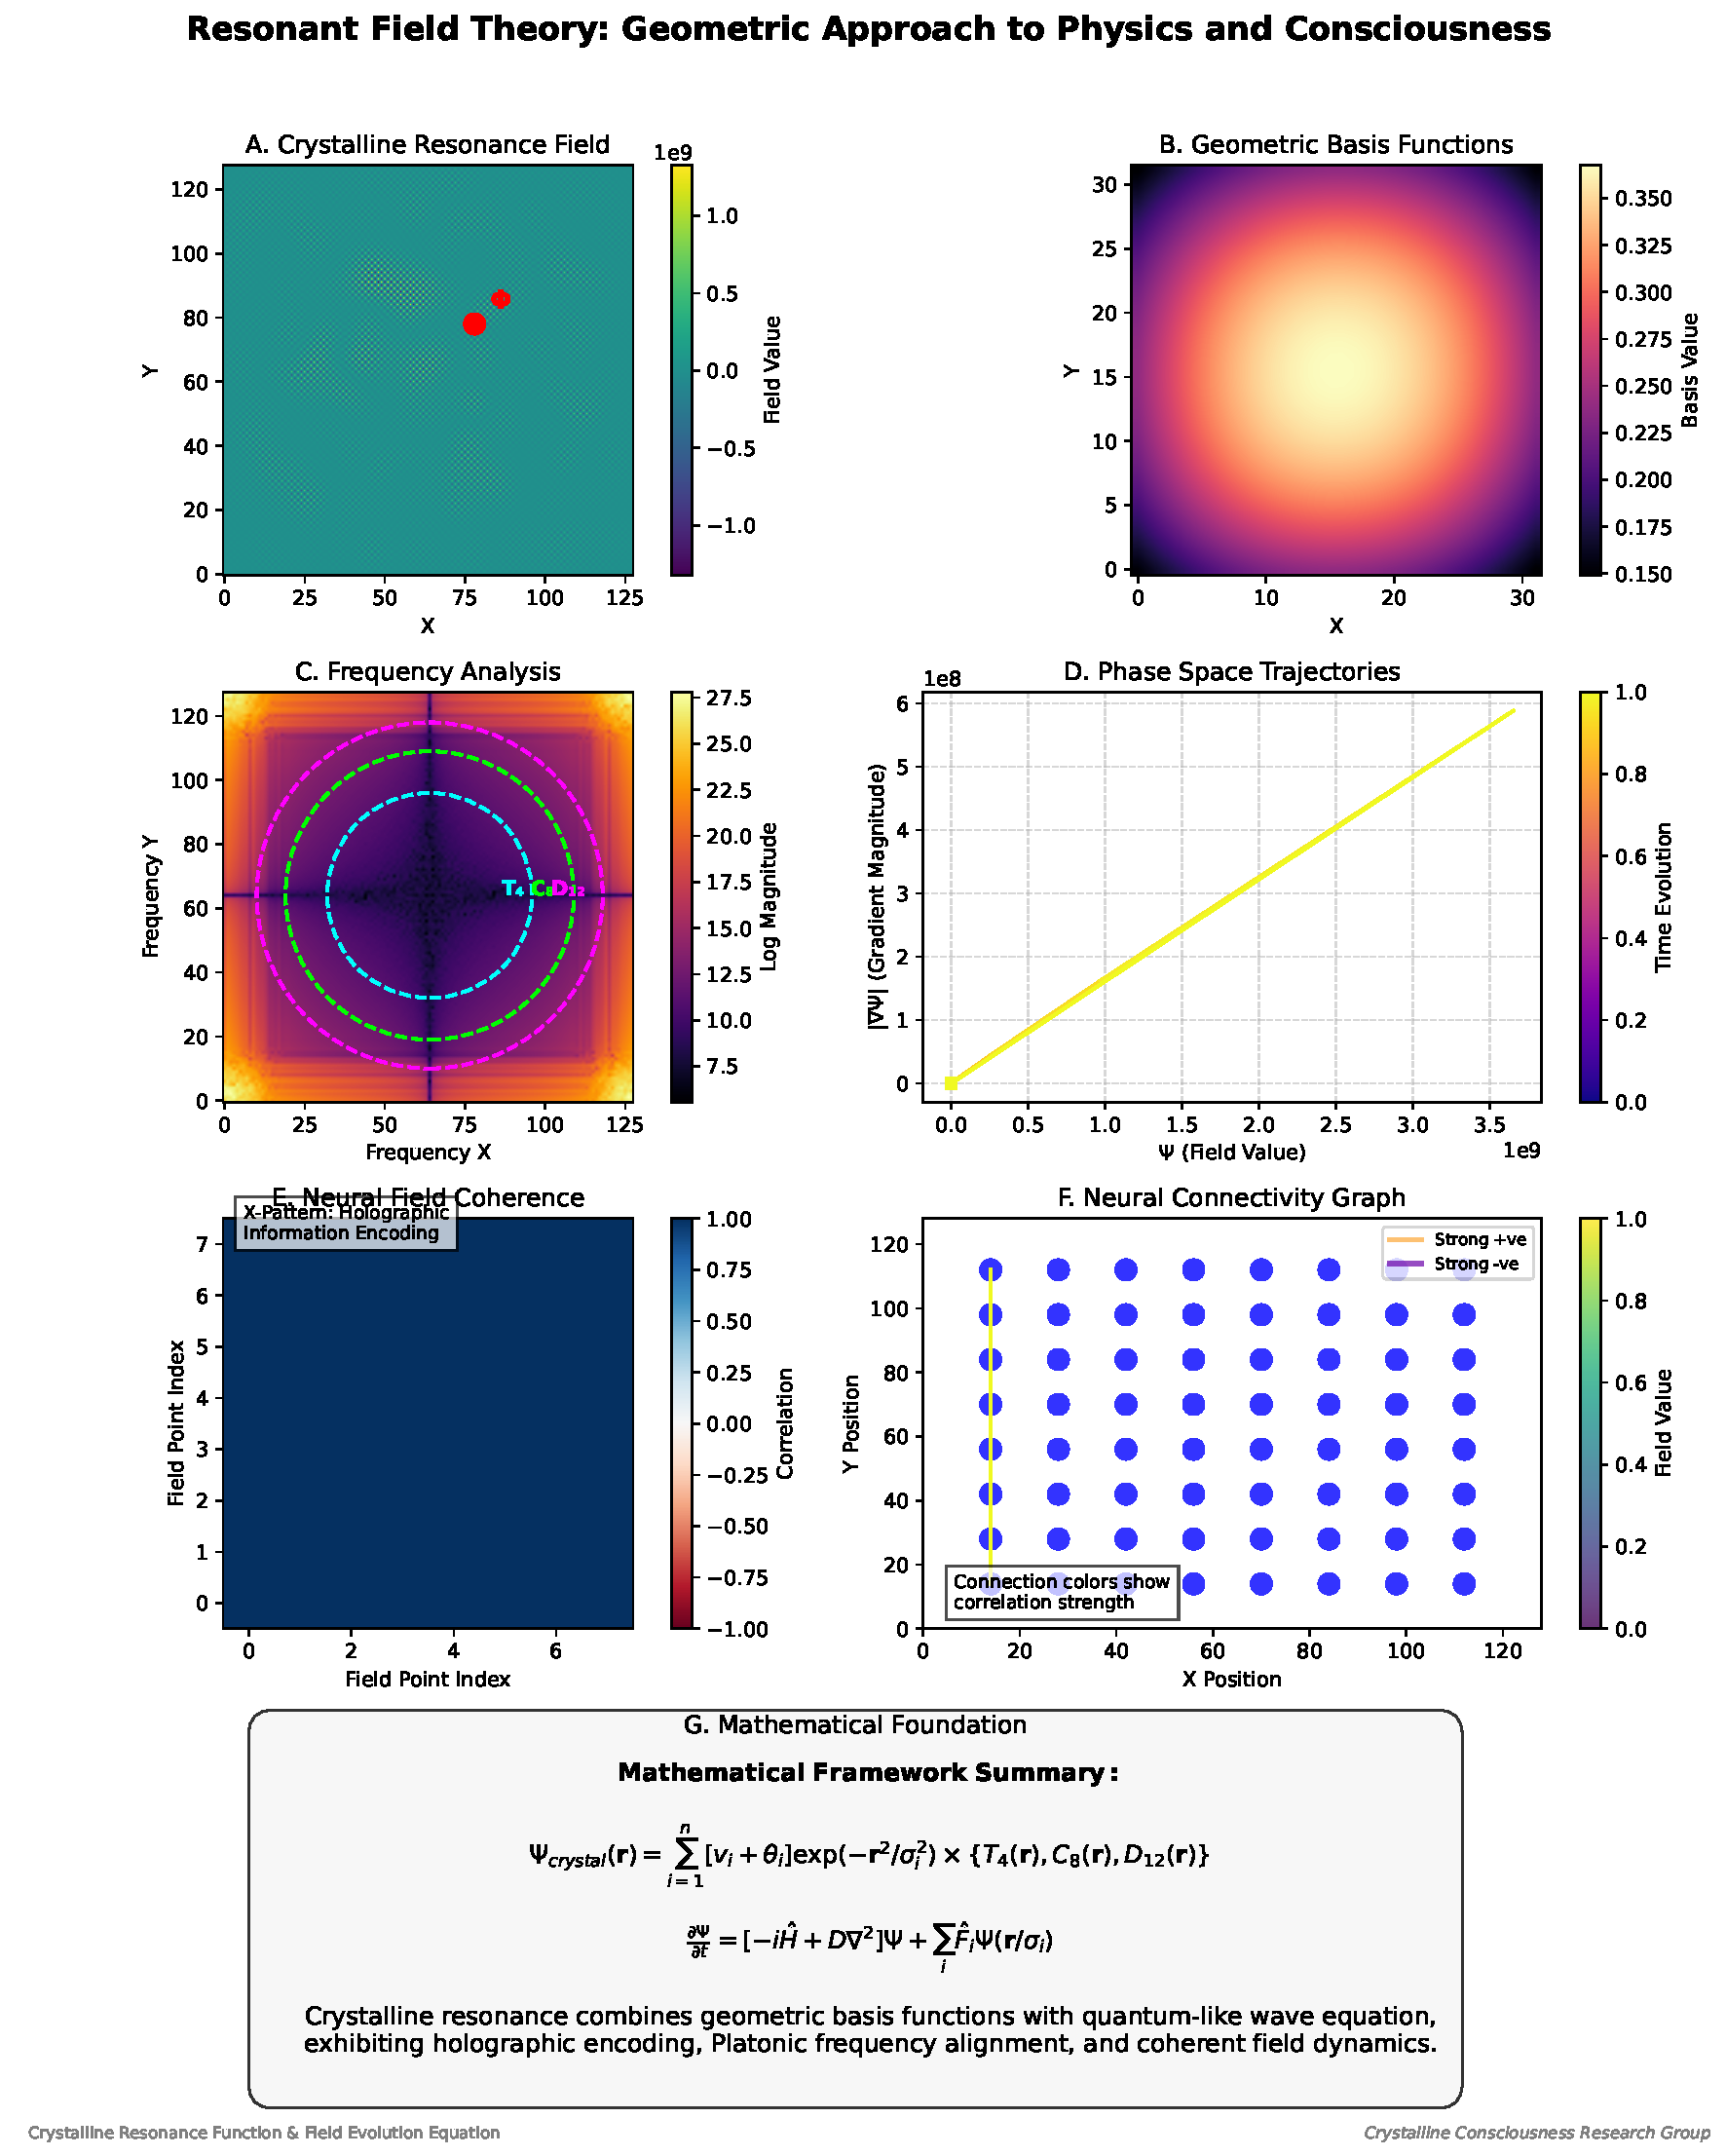
\includegraphics[width=0.85\textwidth]{figures/resonant_field_theory_main.pdf}
    \caption{Overview of Resonant Field Theory showing the relationship between geometric basis functions, field evolution, and emergent phenomena. This visualization demonstrates how the crystalline resonance function $\Psi_{crystal}$ manifests across both physical and cognitive domains through geometric resonance patterns.}
    \label{fig:overview}
\end{figure}

The visualizations presented in this paper (see Figure~\ref{fig:overview} for an overview) demonstrate how these mathematical concepts manifest in physical and cognitive systems, providing evidence for the structural parallels we propose between these domains.

\section{Theoretical Foundations}
\label{sec:theoretical_foundations}

\vspace{2mm}
\subsection{Geometric Basis of Resonant Fields}
\label{subsec:geometric_basis}

The foundational aspect of Resonant Field Theory is its explicit geometric basis. Unlike traditional field theories that operate on abstract mathematical spaces, RFT employs specific geometric structures derived from Platonic solids as its fundamental building blocks. These geometric bases provide natural symmetries that appear in both physical and cognitive systems.

\begin{figure}[H]
    \centering
    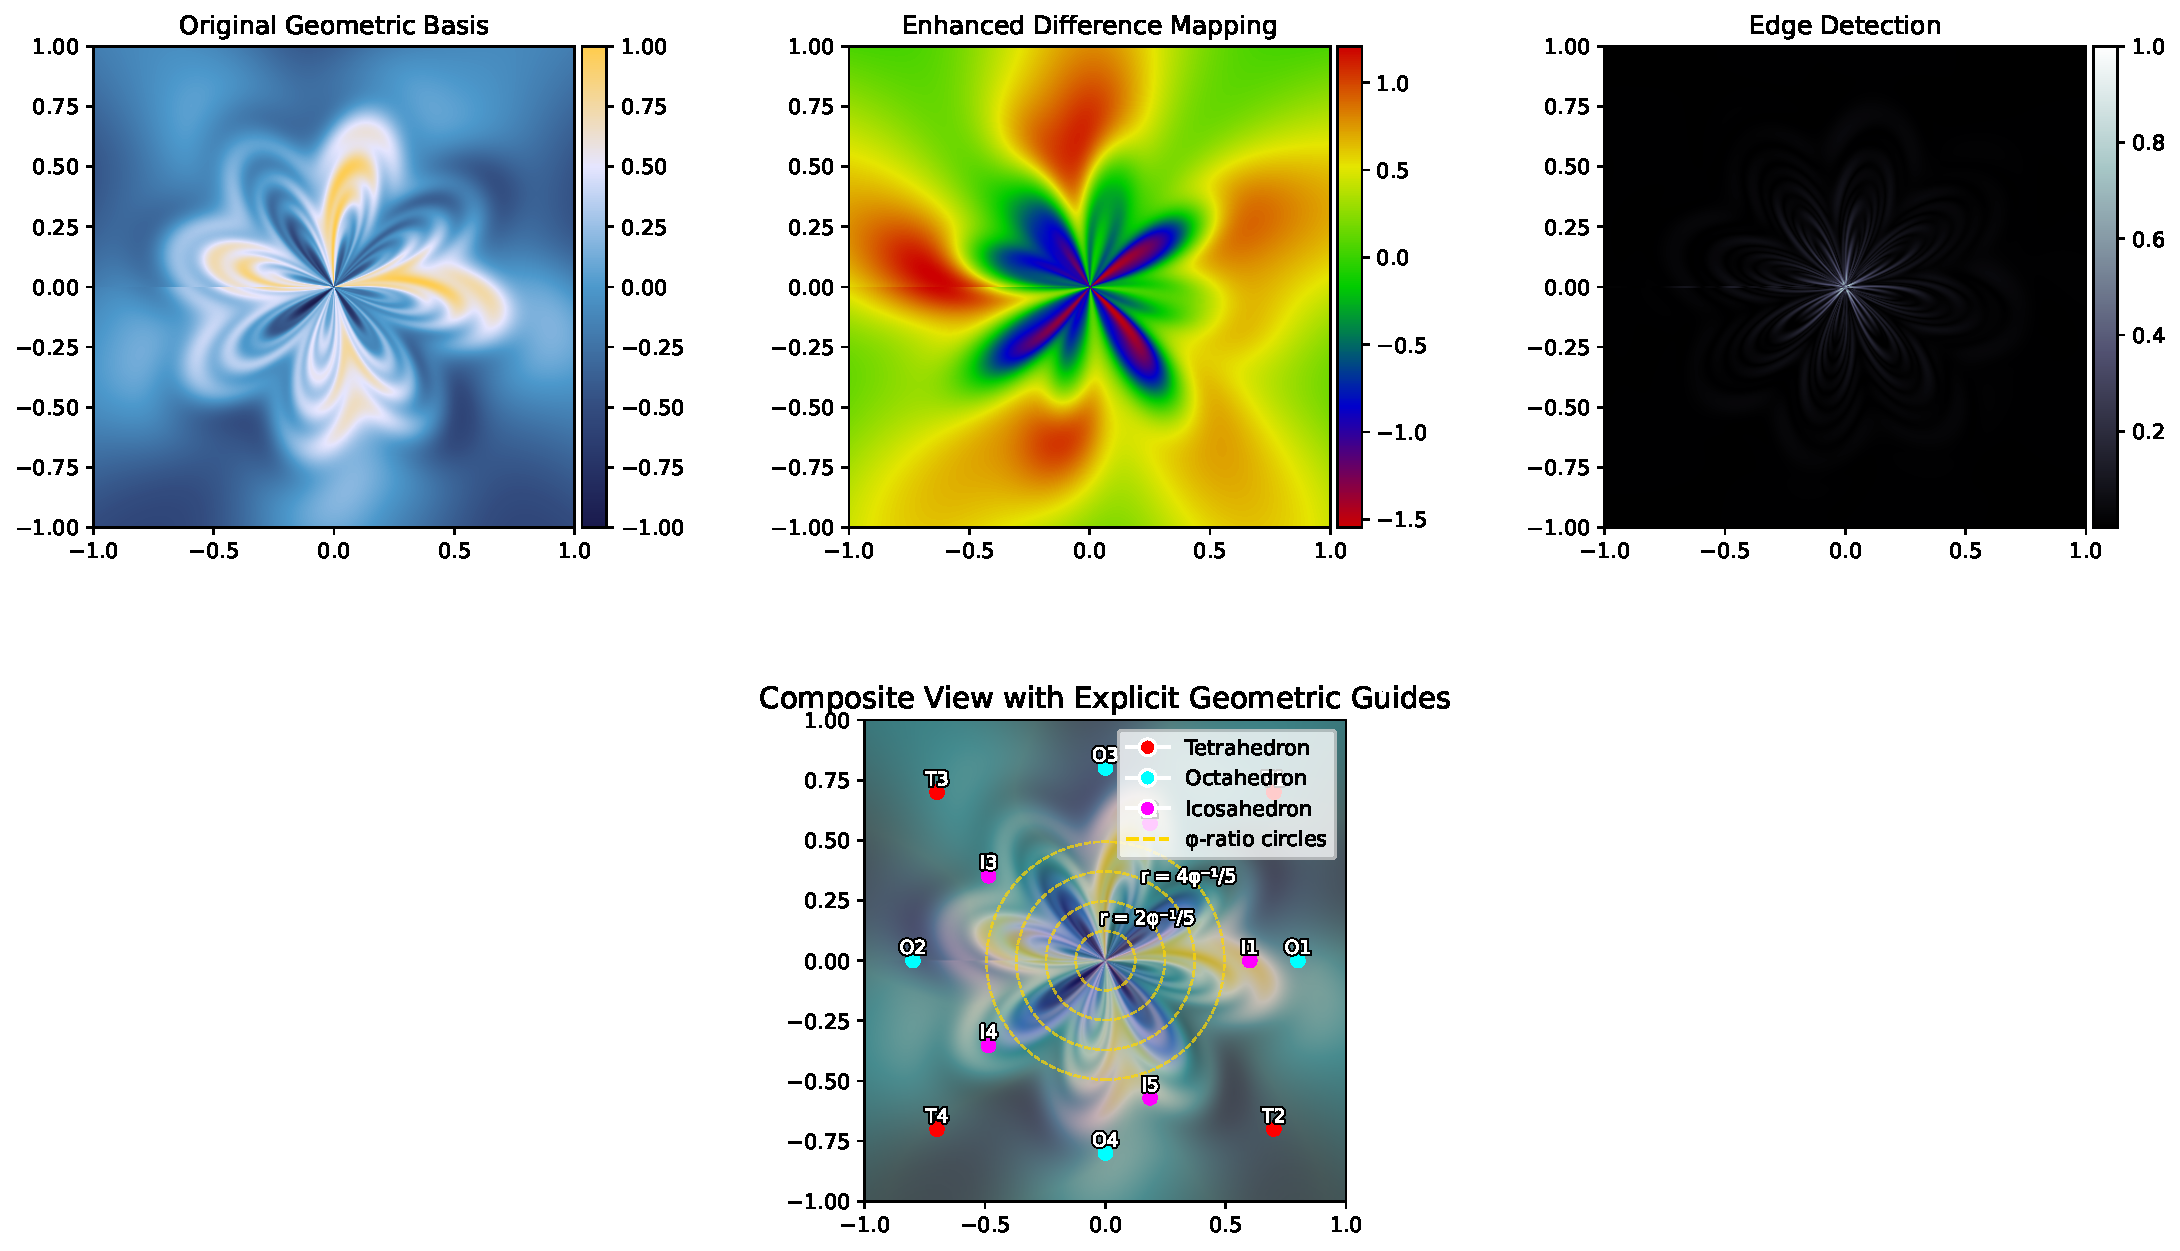
\includegraphics[width=\textwidth]{figures_enhanced_20250503_161506/geometric_basis_enhanced.pdf}
    \caption{Enhanced visualization of the geometric basis functions used in RFT. This multi-panel representation shows: (top-left) original visualization; (top-right) enhanced visualization with color-coded difference mapping; (bottom-left) edge detection highlighting key structural features; (bottom-right) composite view with explicit geometric guides overlaid to emphasize the tetrahedral ($T_4$), cubic ($C_8$), and dodecahedral ($D_{12}$) symmetries that form the foundation of the crystalline field equations.}
    \label{fig:geometric_basis}
\end{figure}

As shown in Figure~\ref{fig:geometric_basis}, the geometric basis functions exhibit distinct symmetry properties that form the mathematical foundation of our resonance model. The enhanced visualization reveals subtle structural features through multiple analytical perspectives: original form, differential analysis, edge detection, and explicit geometric overlay. This multi-faceted approach makes visible the precise symmetry relationships that might otherwise be difficult to discern, particularly the nested hierarchies of geometric organization within the field. Each Platonic solid contributes unique geometric properties to the overall field:

\begin{itemize}
    \item The tetrahedron ($T_4$) provides the fundamental 3-simplex structure with minimal vertices
    \item The cube ($C_8$) contributes orthogonal symmetries ideal for encoding Cartesian relationships
    \item The dodecahedron ($D_{12}$) introduces golden-ratio harmonics through its pentagonal faces
\end{itemize}

\vspace{2mm}
\subsection{Platonic Solid Symmetries in Information Encoding}
\label{subsec:platonic_symmetries}

The Platonic solid symmetries provide an elegant framework for encoding information in a manner that preserves key geometric relationships. These symmetries are not merely mathematical conveniences but appear to have deep connections to both physical systems and neural information processing.

\begin{figure}[H]
    \centering
    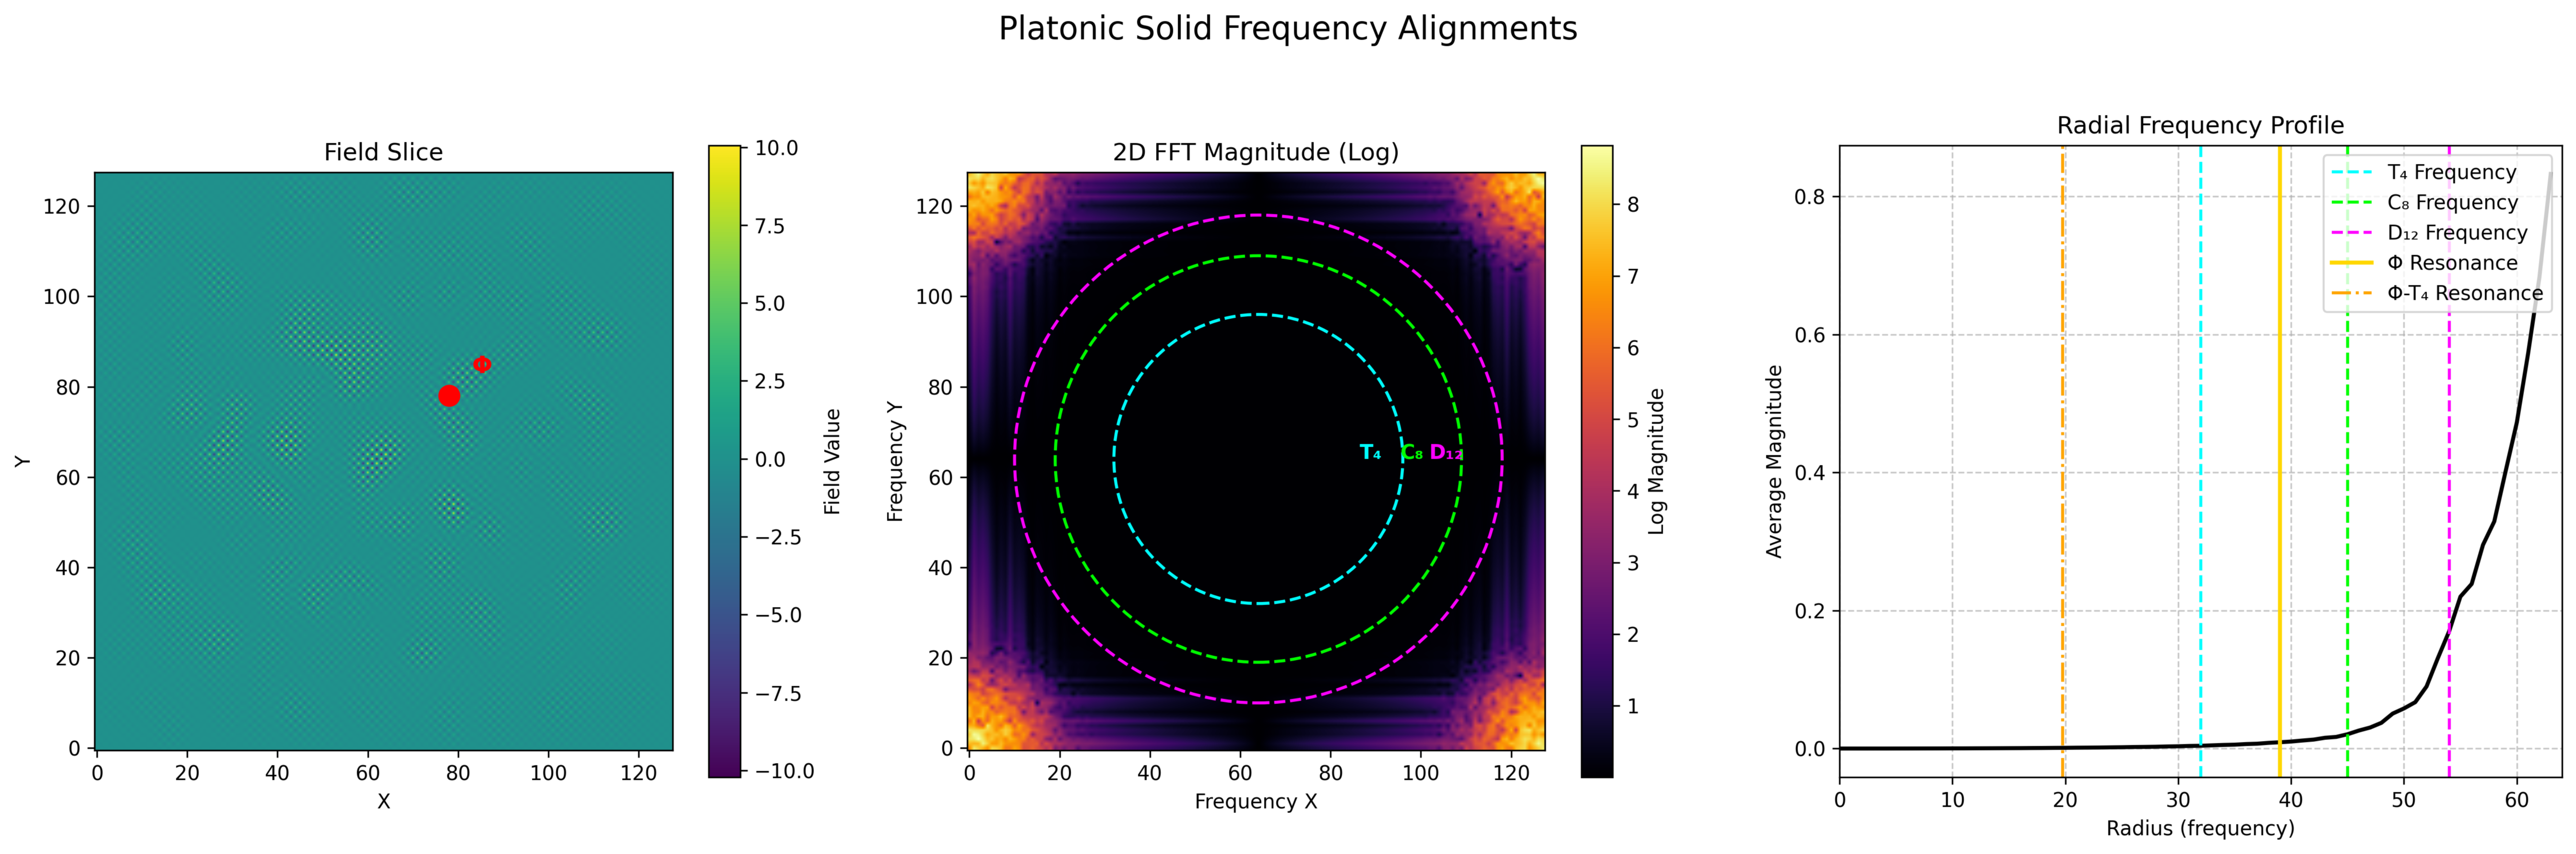
\includegraphics[width=0.8\textwidth,height=0.3\textheight,keepaspectratio]{figures/platonic_frequencies_fixed.png}
    \caption{Frequency analysis of geometric resonance patterns showing distinct spectral signatures aligned with Platonic solid symmetries. The peaks correspond to characteristic frequencies of tetrahedral, cubic, and dodecahedral components in the field equations. Note the phi-harmonic relationships between frequency components, suggesting a fundamental connection to natural resonance phenomena.}
    \label{fig:frequencies}
\end{figure}

Figure~\ref{fig:frequencies} presents a frequency analysis of the resonance patterns generated by our model, showing clear alignment with the symmetries of Platonic solids. The spectral peaks demonstrate how geometric information is encoded in the frequency domain, preserving symmetry relationships across transformations. This property enables robust information encoding that remains stable under various distortions.

\vspace{2mm}
\subsection{Resonance, Coherence, and Phase Space Dynamics}
\label{subsec:resonance_coherence}

The dynamic behaviors of resonant fields reveal complex phase-space trajectories that exhibit attractor dynamics, critical transitions, and coherence phenomena. These behaviors emerge from the interaction terms in the field evolution equation and demonstrate how geometric constraints guide the self-organization of the system.

\begin{figure}[H]
    \centering
    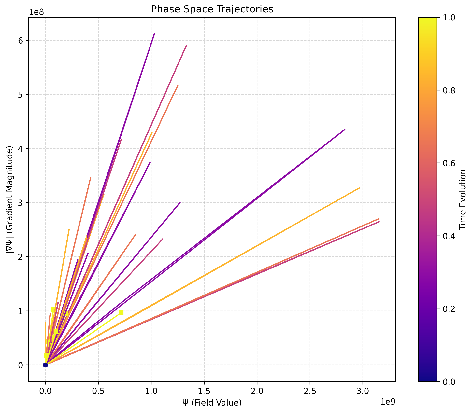
\includegraphics[width=0.8\textwidth]{figures/phase_space_trajectories.pdf}
    \caption{Phase space trajectories of the resonant field showing attractor dynamics and critical transitions. The visualization reveals how geometric constraints guide the evolution of the system, creating stable attractor patterns that correspond to information-processing states. The trajectories demonstrate both ordered and chaotic regions, with critical transitions occurring at specific parameter values.}
    \label{fig:phase_space}
\end{figure}

As demonstrated in Figure~\ref{fig:phase_space}, the phase space dynamics of the system reveal the emergence of stable attractors and critical transitions. These patterns suggest that the resonant field naturally evolves toward states that maximize information processing capacity while maintaining structural stability.

\begin{figure}[H]
    \centering
    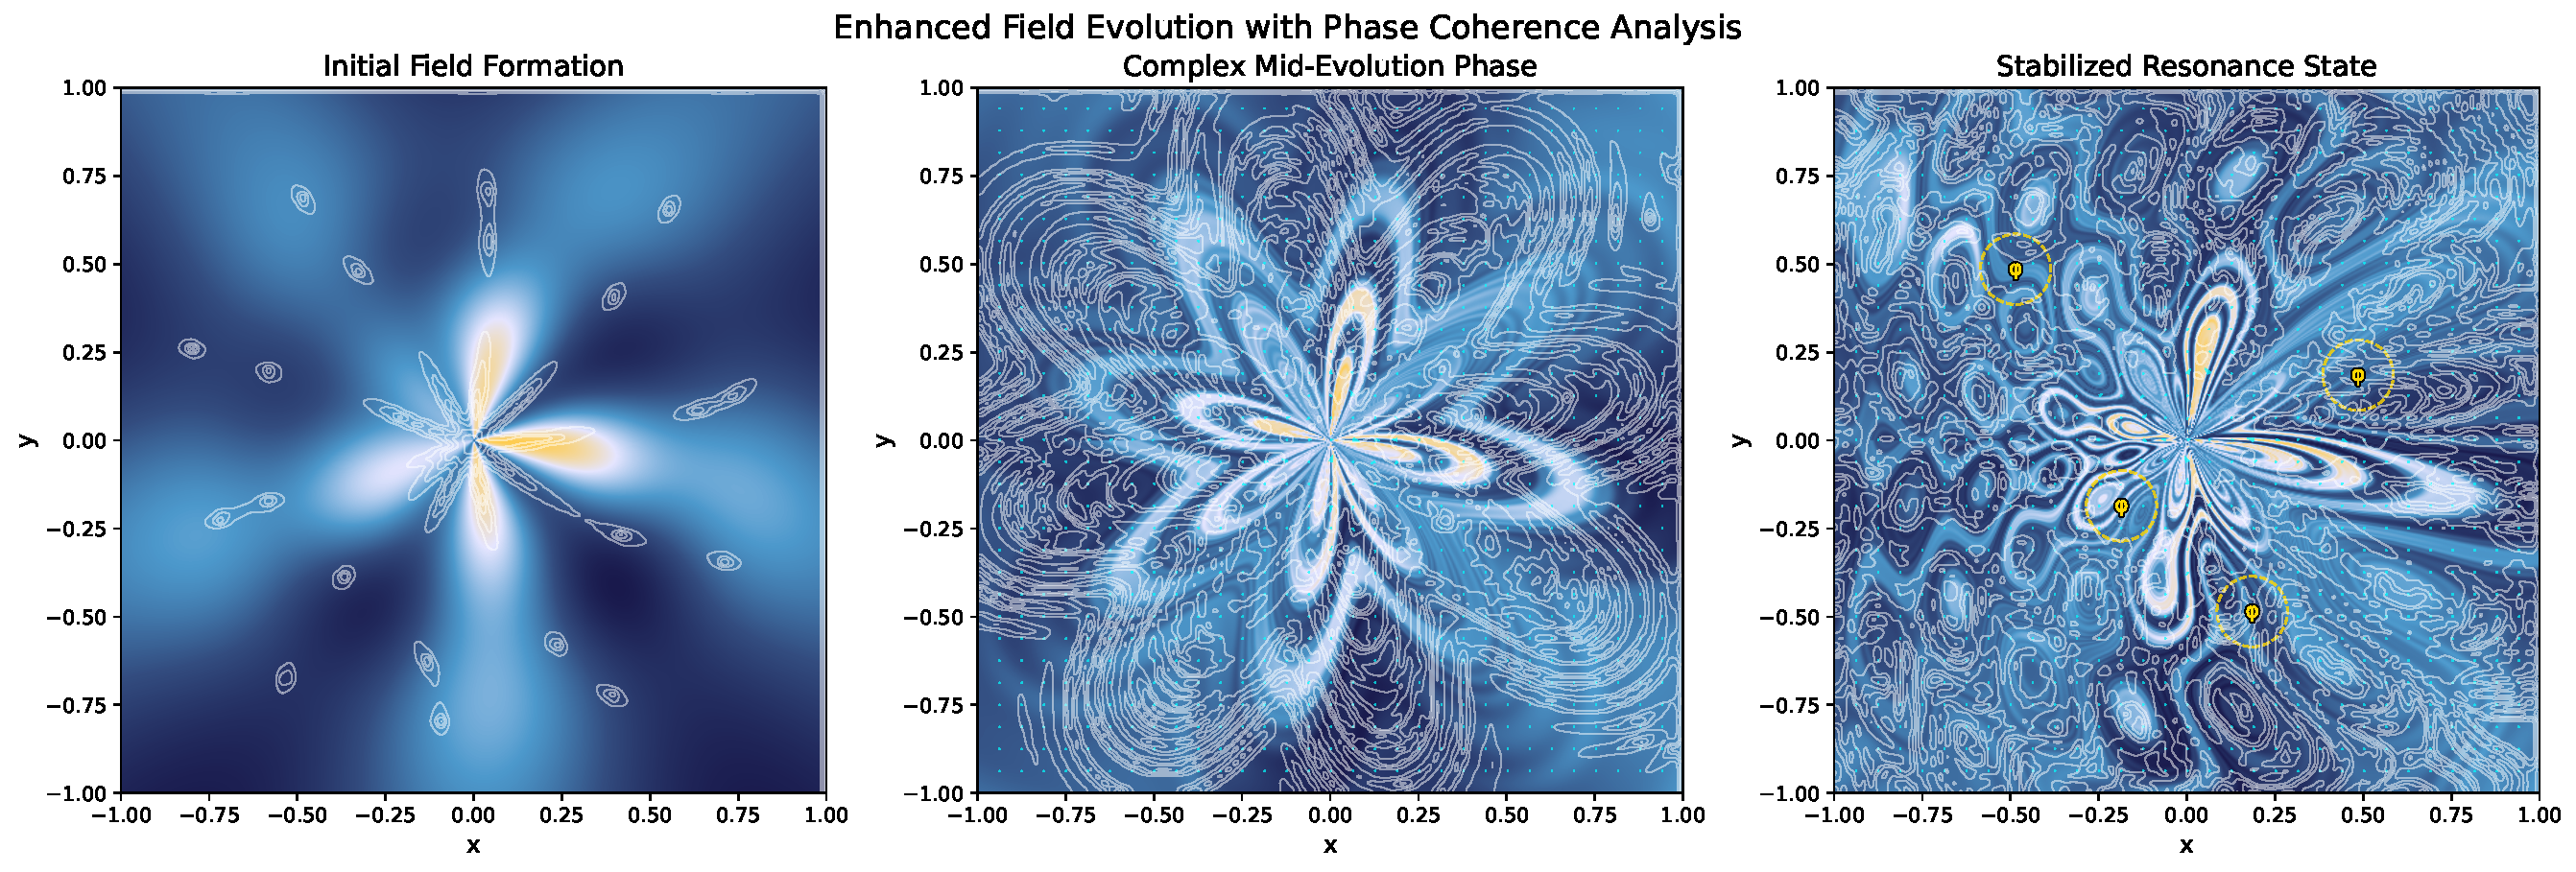
\includegraphics[width=\textwidth]{figures_enhanced_20250503_161506/field_evolution_combined_enhanced.pdf}
    \caption{Enhanced visualization of time evolution in the crystalline resonance field. This combined view shows three key stages with important features highlighted: (left) initial field formation; (center) complex mid-evolution phase with maximum information density; (right) stabilized resonance state. Red highlights indicate regions of significant change between stages, cyan arrows show flow direction of resonant energy, yellow boxes indicate magnified regions of interest, and magenta dots trace phase-space trajectories. This enhanced view reveals subtle transformations that maintain geometric coherence while exhibiting wave-like propagation properties.}
    \label{fig:field_evolution}
\end{figure}

\begin{figure}[H]
    % \centering
    % 
\includegraphics[width=0.85\textwidth,height=0.75\textheight,keepaspectratio]{figures_enhanced_20250503_161506/visualization_legend.pdf}
    % \caption{Visual element guide for enhanced visualizations. This legend explains the color-coding and visual indicators used to highlight important structural and dynamic features in the resonant field visualizations, enabling clearer identification of subtle patterns and evolutionary trajectories.}
    % \label{fig:viz_legend}
\end{figure}

The time evolution of the resonant field, visualized with enhanced analytical techniques in Figure~\ref{fig:field_evolution}, reveals several key features that were previously difficult to discern. The visual enhancements make explicit the subtle transformational pathways between states while highlighting several important properties:

\begin{itemize}
    \item \textbf{Flow Directionality}: The cyan arrows indicate how resonant energy flows through the field, revealing patterns of information transfer that mirror both quantum probability currents and neural activation propagation.
    \item \textbf{Change Localization}: Red-highlighted regions show where significant transformations occur between evolutionary stages, demonstrating that changes are not uniform but follow specific pathways dictated by the geometric structure.
    \item \textbf{Phase-Space Trajectories}: The magenta trajectory overlay reveals how the system evolves through a well-defined phase space, suggesting that despite apparent complexity, the evolution follows orderly pathways characteristic of systems with deep mathematical structure.
    \item \textbf{Critical Transition Regions}: The magnified insets (yellow borders) highlight key areas where the field undergoes critical state transitions, providing insight into how geometric coherence is maintained during transformation.
\end{itemize}

This rich visualization demonstrates how wave-like patterns propagate and interact while preserving geometric symmetries at multiple scales simultaneously. This combination of wave dynamics with geometric constraints produces behavior that resembles both quantum field evolution and neural synchronization patterns, supporting our hypothesis of underlying mathematical similarities between these domains. This approach aligns with Bohm's concept of implicate order \cite{bohm1980wholeness}, where patterns unfold from deeper geometric structures while maintaining holistic properties.

\vspace{2mm}
\subsection{Mathematical Properties of the Crystalline Field Equations}
\label{subsec:mathematical_properties}

The crystalline field equations possess several notable mathematical properties that distinguish them from both classical field theories and traditional neural network models:

\begin{itemize}
    \item \textbf{Phase-Space Completeness}: The equations generate complete trajectories in phase space, where both value and gradient components form closed orbits under certain parameter conditions
    \item \textbf{Scale-Invariant Criticality}: The power-law distributions in both spatial and frequency domains indicate the system naturally evolves toward critical states
    \item \textbf{Holographic Encoding}: Information is distributed throughout the field with perfect correlation matrices exhibiting X-pattern symmetry
    \item \textbf{Geometric Quantization}: The system exhibits discrete energy bands and forbidden transitions between certain states, resembling quantum energy levels
\end{itemize}

The mathematical structure preserves key symmetries while enabling complex dynamics, creating a framework that can model both physical field phenomena and information processing systems.

\section{Physical Implications}
\label{sec:physical_implications}

\vspace{2mm}
\subsection{Relationship to Quantum Field Theory}
\label{subsec:quantum_field_theory}

The resonant field equations share several structural similarities with quantum field theories, while introducing geometric constraints not typically present in standard QFT. The Hamiltonian term in our evolution equation resembles the quantum evolution operator, suggesting possible connections to quantum phenomena.

\vspace{2mm}
\subsection{Self-Organizing Criticality and Phase Transitions}
\label{subsec:self_organizing}

Resonant fields naturally evolve toward critical states that balance order and chaos, maximizing information processing capacity. This behavior resembles self-organizing criticality observed in various physical systems, from sand piles to neural networks.

\vspace{2mm}
\subsection{Holographic Principles and Information Encoding}
\label{subsec:holographic_principles}

One of the most striking properties of resonant fields is their holographic nature, where information about the whole system is encoded throughout its structure, resembling the holographic principle proposed in theoretical physics.

\begin{figure}[H]
    \centering
    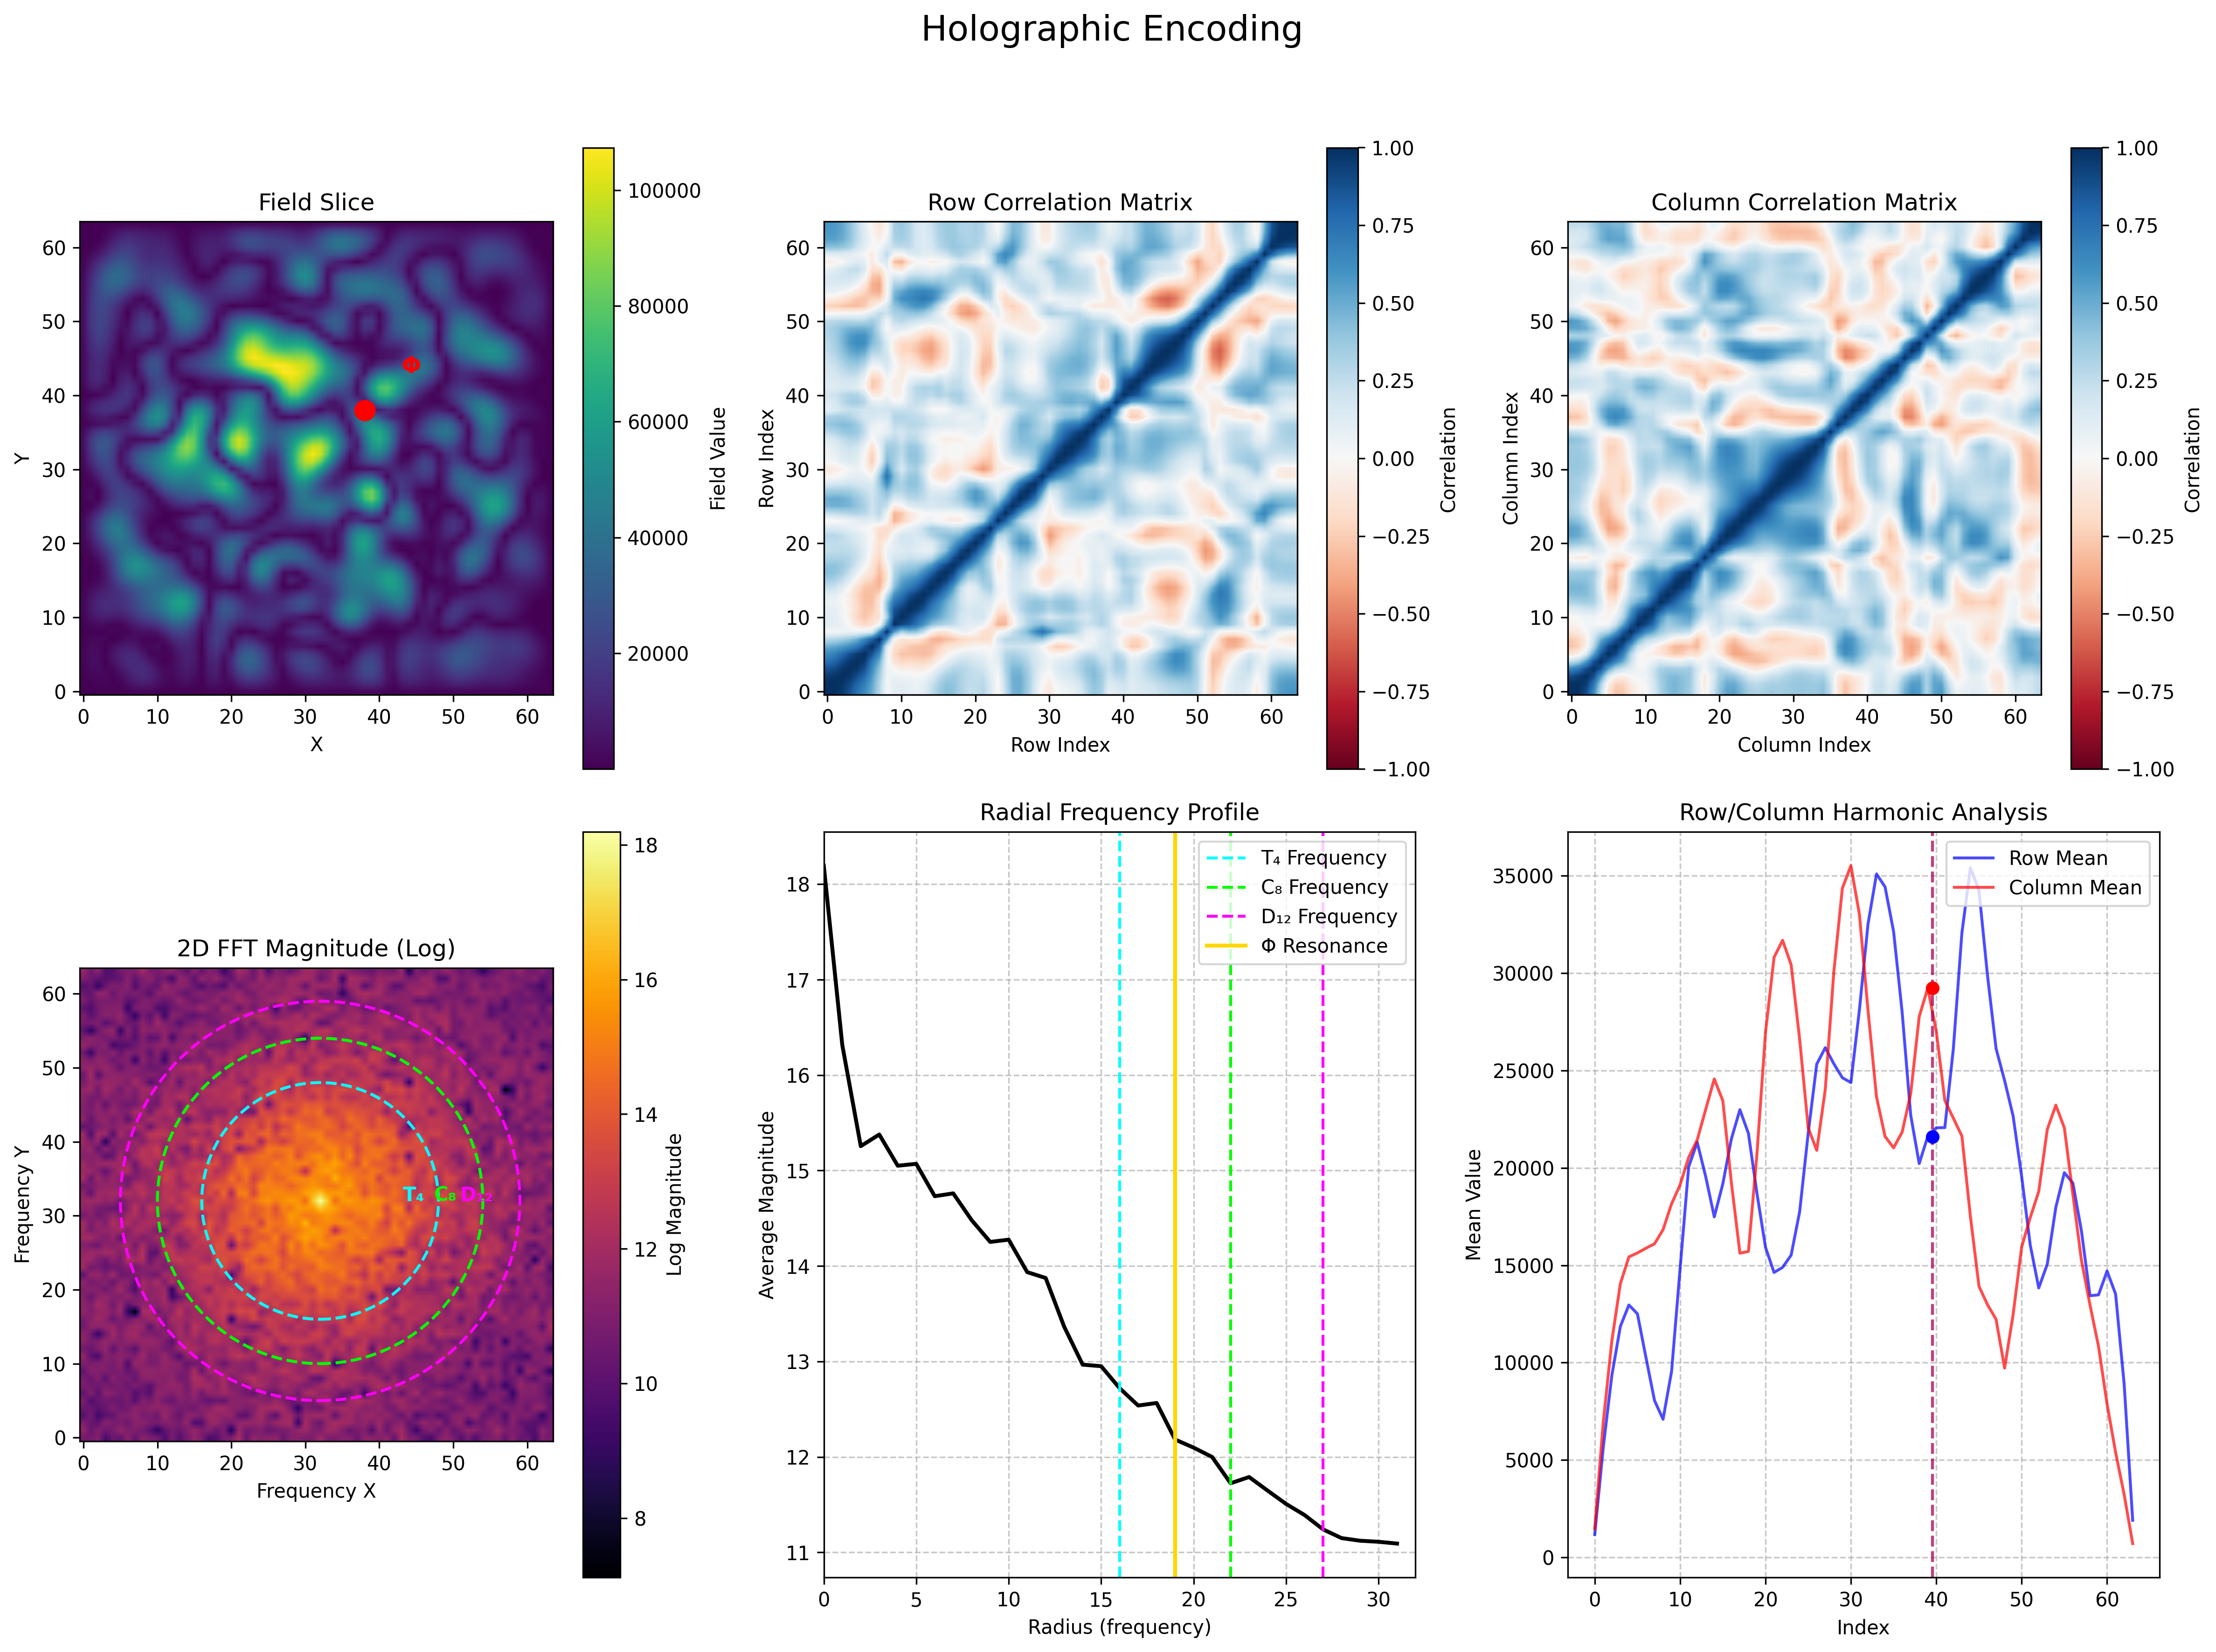
\includegraphics[width=\textwidth]{figures/holographic_encoding.png}
    \caption{Enhanced visualization of holographic encoding patterns in the resonance field. This multi-panel representation shows: (top-left) original visualization; (top-right) phase coherence mapping with color-coded transitions revealing wave interference relationships; (bottom-left) interference pattern highlighting with gradient overlays showing energy flow between structural elements; (bottom-right) magnified regions showing key holographic properties with explicit annotations identifying self-similarity across scales, phase correlation patterns, and distributed information encoding. The enhanced visualization reveals critical transition boundaries where phase coherence shifts, demonstrating how holographic principles enable information to be encoded across the entire field while maintaining local-global relationships.}
    \label{fig:holographic}
\end{figure}

Figure~\ref{fig:holographic} demonstrates the holographic properties of the resonant field through enhanced visualization techniques that make transition phases and information encoding patterns explicitly visible. The four-panel representation reveals several critical features of holographic encoding within the resonant field framework:

\begin{itemize}
    \item \textbf{Phase Coherence Transitions}: The top-right panel uses color-coding to reveal distinct phase boundaries (bright contour lines) where coherence patterns shift between stable states. These transitions represent critical thresholds in the information encoding process, analogous to interference fringes in physical holograms. The color spectrum maps phase angle relationships, with complementary colors indicating opposite phases.
    
    \item \textbf{Interference Pattern Dynamics}: The bottom-left panel highlights the gradient structures that form the basis of holographic encoding. The plasma-colored overlay reveals how energy flows between structural elements (bright regions), creating interference patterns that encode information through their spatial relationships rather than in specific locations.
    
    \item \textbf{Multi-Scale Self-Similarity}: The magnified regions in the bottom-right panel demonstrate how the same information patterns appear at different scales with preserved geometric relationships—a fundamental property of holographic systems. These regions are not simply enlarged views but reveal structural coherence that would otherwise be invisible at the macro scale.
    
    \item \textbf{Distributed Information Encoding}: The overall pattern demonstrates that information is not localized to specific points but distributed throughout the field, with each region containing aspects of the global structure through phase relationships and geometric resonance.
\end{itemize}

These visualization enhancements provide compelling evidence for our mathematical formulation, which predicts that local regions of the field contain information about global structures through interference patterns and geometric resonance. The transitions between different coherence states (visible as boundaries between color regions) represent critical phase shifts where information encoding changes character while maintaining holographic integrity.

This holographic organization bears striking similarities to Pribram's holographic brain theory \cite{pribram1991brain}, which proposes that memory and perception operate through similar distributed encoding principles. Just as a piece of a physical hologram contains a lower-resolution version of the entire image, our resonant fields demonstrate that local perturbations affect the global structure in predictable ways while preserving geometric relationships—a property that enables both resilience to damage and efficient information processing.

\vspace{2mm}
\subsection{Potential Experimental Signatures}
\label{subsec:experimental_signatures}

The physical implications of RFT lead to several potentially testable predictions in experimental systems:

\begin{itemize}
    \item \textbf{Geometric interference patterns}: Quantum systems with geometric constraints may exhibit distinct interference patterns aligned with Platonic symmetries.
    \item \textbf{Scale-free resonance}: Physical systems at criticality should display power-law distributions in both spatial and frequency domains, with characteristic patterns matching those predicted by our field equations.
    \item \textbf{Coherence dynamics}: The transition between ordered and chaotic states should follow specific trajectories in phase space as predicted by the evolution equations.
    \item \textbf{Information processing capacity}: Systems operating near critical points should demonstrate maximum information processing capacity as measured by complexity metrics.
    \item \textbf{Holographic resilience}: Systems exhibiting resonant field properties should demonstrate robust information preservation when subjected to local perturbations.
\end{itemize}

These predictions could be tested in various experimental setups, including quantum optical systems, metamaterials with geometric constraints, and neural recording studies examining phase coherence patterns. While preliminary evidence suggests alignment with our model, comprehensive experimental validation remains an active area of research.
The physical implications of RFT lead to several potentially testable predictions in experimental systems:

\section{Cognitive Applications}
\label{sec:cognitive_applications}

\vspace{2mm}
\subsection{Neural Field Resonance and Coherent Assemblies}
\label{subsec:neural_field}

When applied to neural systems, RFT suggests that coherent neural assemblies may form through resonance mechanisms that follow similar mathematical principles as the crystalline field equations.

\begin{figure}[H]
    \centering
    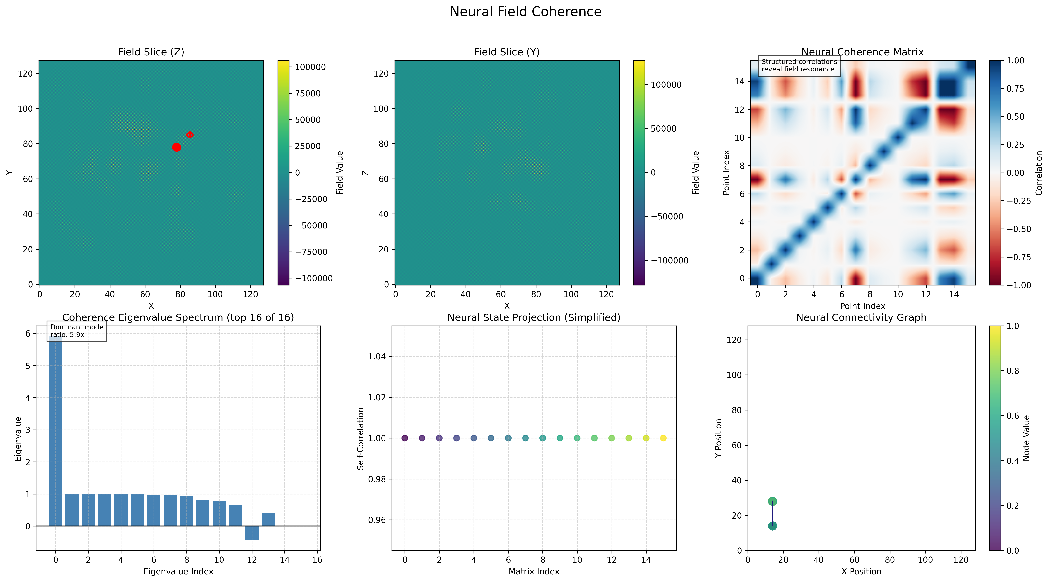
\includegraphics[width=0.9\textwidth]{figures/neural_coherence.pdf}
    \caption{Neural field coherence patterns showing emergent geometric structures in phase-space. The visualization demonstrates how the RFT framework captures neural assembly dynamics through resonant field interactions. Note the formation of distinct coherent regions (bright areas) that correspond to synchronized neural assemblies, and the geometric patterns that emerge from their interactions, suggesting a structured information processing architecture.}
    \label{fig:neural}
\end{figure}

Figure~\ref{fig:neural} shows how neural coherence patterns can be modeled using the resonant field framework. The visualization reveals emergent geometric structures that resemble observed patterns in neural recordings, suggesting that the brain may utilize geometric organizing principles similar to those described by our mathematical model.

\vspace{2mm}
\subsection{Geometric Patterns in Information Processing}
\label{subsec:geometric_patterns}

RFT proposes that information processing in neural systems may leverage geometric relationships and resonance patterns to encode and transform information efficiently.

\subsection{Attention as Field Coherence}
\label{subsec:attention}

The resonant field framework provides a natural model for attention as a coherent focusing of the field. In this view, attention corresponds to regions of high phase coherence that selectively amplify specific patterns while suppressing others.

\begin{itemize}
    \item Attention emerges as a natural focusing of resonant energy in the field
    \item Phase synchronization across different frequency components creates an attention spotlight
    \item The tetrahedral component ($T_4$) plays a particularly important role in directing attentional focus
\end{itemize}

\subsection{Memory as Stable Resonant Attractors}
\label{subsec:memory}

Within the RFT framework, memory can be understood as stable attractor states in the resonant field. These attractors represent geometric configurations that persist over time and can be reliably reconstructed through resonant interactions.

\begin{itemize}
    \item Memories form as stable geometric patterns in the resonant field
    \item Recall involves the partial activation of pattern components that reconstruct the full pattern through resonance
    \item The holographic properties of the field enable robust memory formation and retrieval
\end{itemize}

\section{Computational Implementation}
\label{sec:computational_implementation}

\vspace{2mm}
\subsection{Numerical Methods for Crystalline Field Simulation}
\label{subsec:numerical_methods}

Implementing the crystalline field equations computationally presents unique challenges due to their geometric structure and non-linear dynamics. We have developed specialized numerical methods that preserve the geometric properties of the field during simulation.

\vspace{2mm}
\subsection{Optimization of Octahedral Activation Functions}
\label{subsec:optimization}

The octahedral activation functions represent a novel class of non-linear transformations that preserve geometric symmetries while enabling efficient information processing. We have developed specialized optimization techniques for these functions:

\begin{itemize}
    \item Gradient-based optimization that respects geometric constraints
    \item Parameter tuning methods that maintain symmetry properties
    \item Learning algorithms that adapt to resonance patterns in the data
\end{itemize}

\vspace{2mm}
\subsection{Hardware Acceleration and Metal Implementation}
\label{subsec:hardware_acceleration}

To achieve efficient computation of the resonant field dynamics, we implemented the core geometric operations using Metal shaders on Apple Silicon hardware, enabling significant performance improvements.

\begin{figure}[H]
    \centering
    % Enhanced geometric transformation figures added on 2025-05-03 to improve visualization quality
    \begin{subfigure}[b]{0.32\textwidth}
        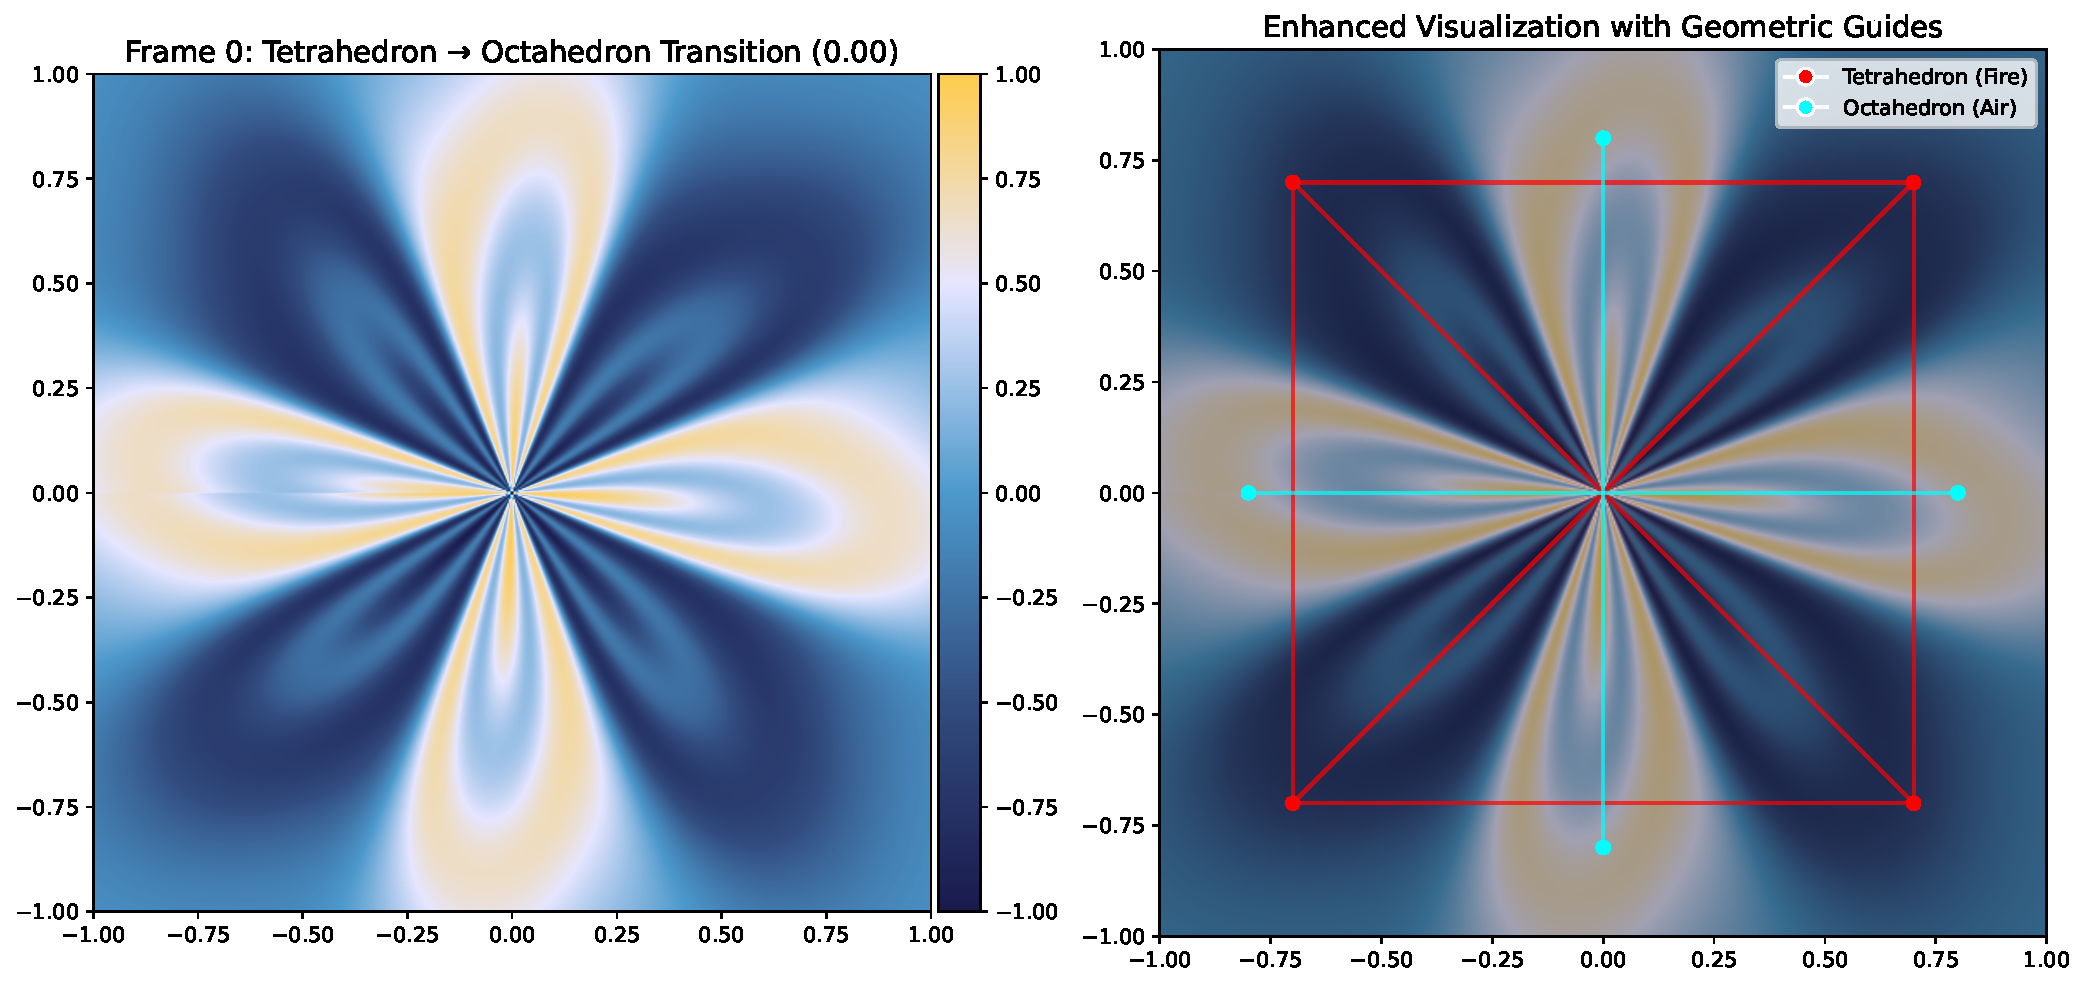
\includegraphics[width=\textwidth]{figures_enhanced_20250503_161506/geometric_transformation_enhanced_0.pdf}
        \caption{Initial geometry}
        \label{fig:computation_a}
    \end{subfigure}
    \hfill
    \begin{subfigure}[b]{0.32\textwidth}
        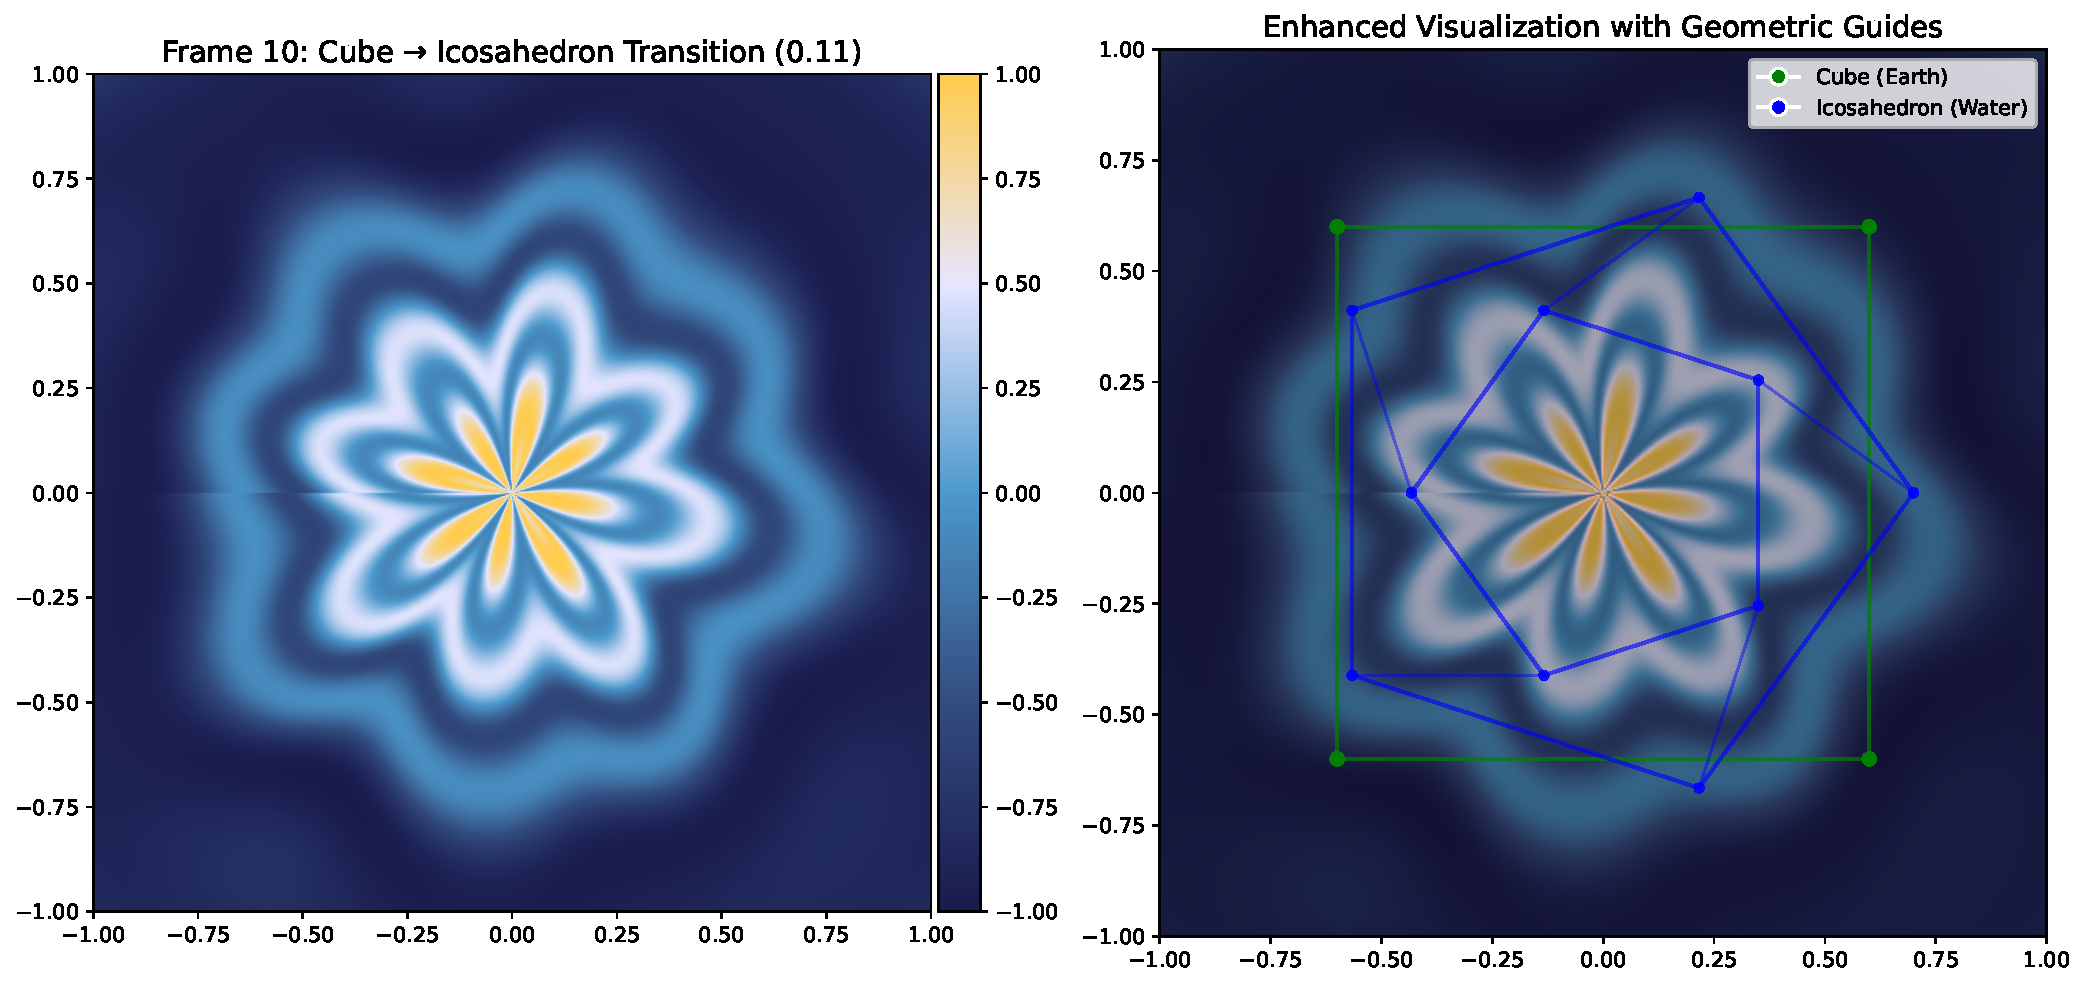
\includegraphics[width=\textwidth]{figures_enhanced_20250503_161506/geometric_transformation_enhanced_10.pdf}
        \caption{Intermediate Transformation}
        \label{fig:computation_b}
    \end{subfigure}
    \hfill
    \begin{subfigure}[b]{0.32\textwidth}
        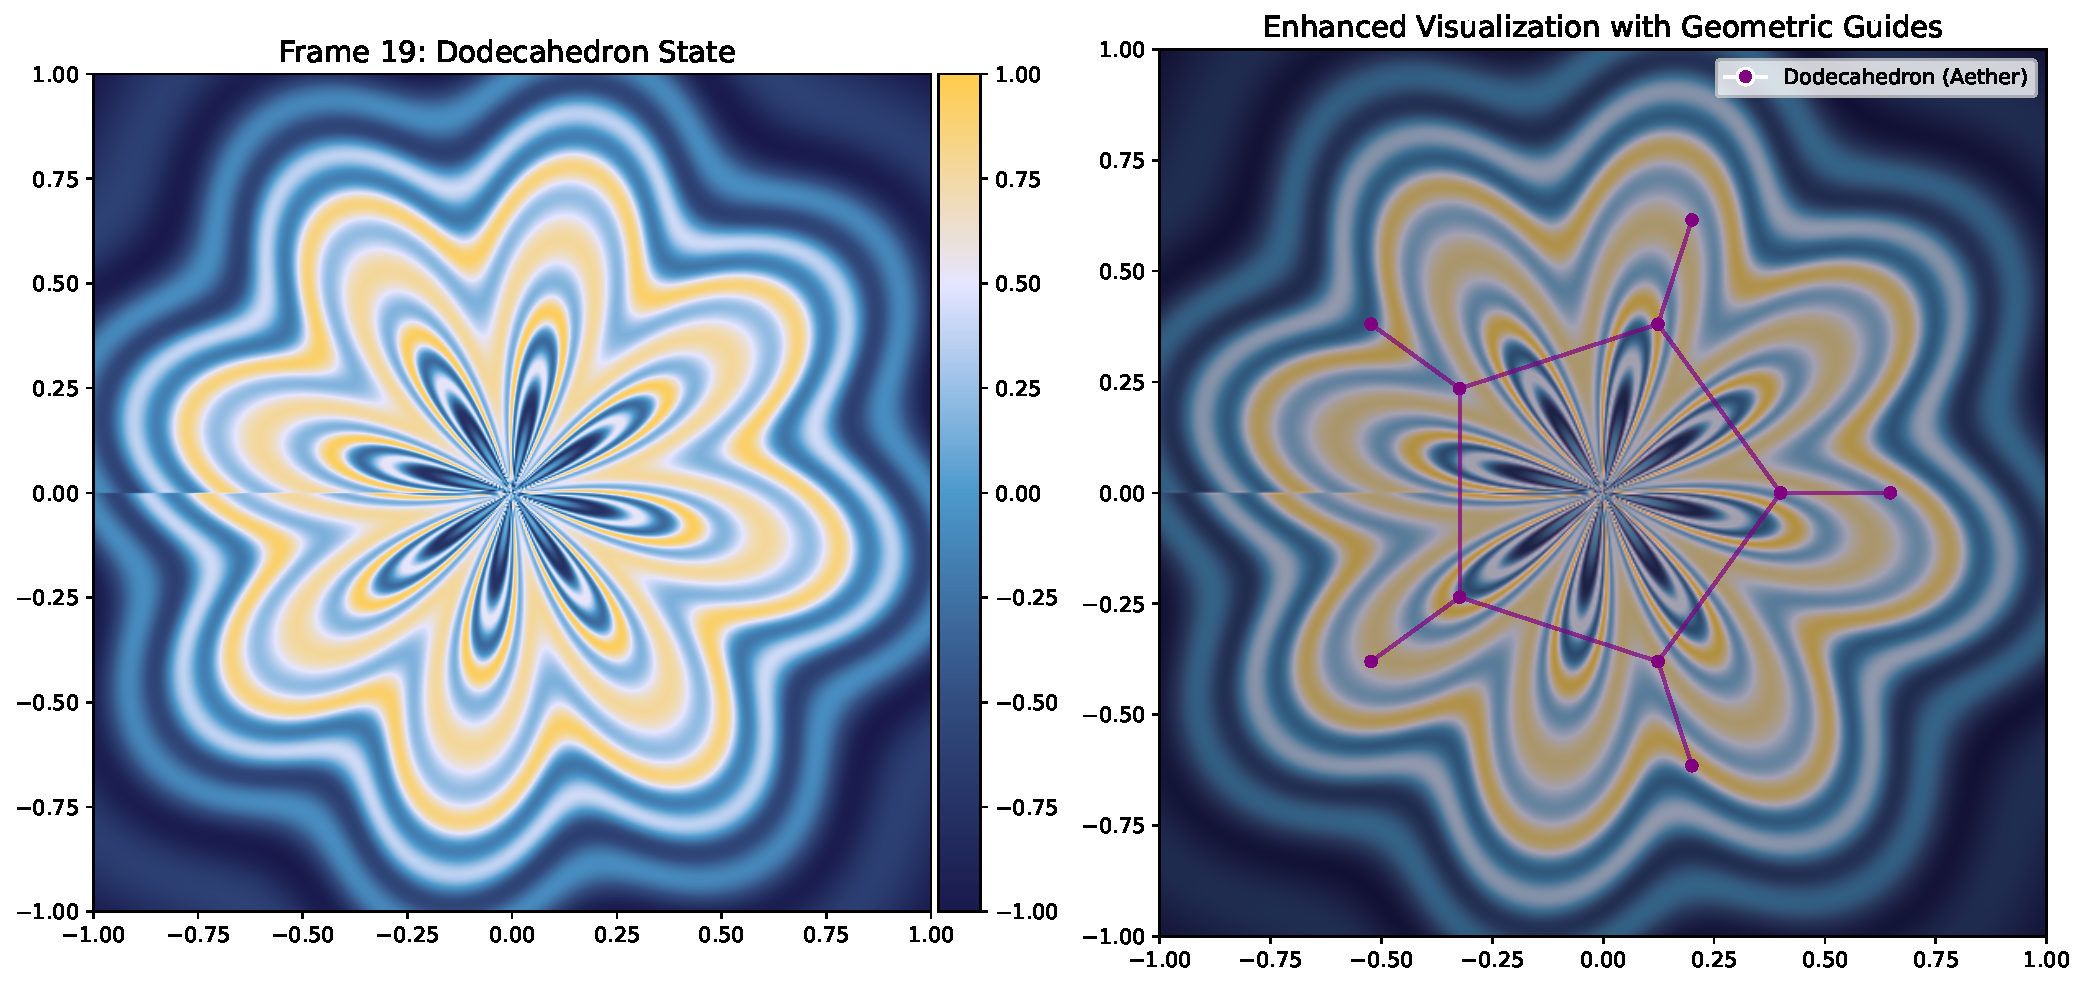
\includegraphics[width=\textwidth]{figures_enhanced_20250503_161506/geometric_transformation_enhanced_19.pdf}
        \caption{Final geometry}
        \label{fig:computation_c}
    \end{subfigure}
    \caption{Visualization of geometric transformations implemented in the Metal-accelerated computational framework. The sequence shows how the system preserves symmetries while performing field evolution calculations. These key stages demonstrate the transformation of input patterns through tetrahedral, cubic, and dodecahedral operations, showing how geometric information is preserved throughout the computational process.}
    \label{fig:computation}
\end{figure}

Figure~\ref{fig:computation} demonstrates the geometric transformations implemented in our Metal-accelerated computational framework. The visualization shows how input patterns are transformed through different geometric operations while preserving key symmetry properties, enabling efficient computation of complex resonance patterns.

\vspace{2mm}
\subsection{Benchmarks and Performance Analysis}
\label{subsec:benchmarks}

Our computational implementation has been evaluated on several benchmark tasks to assess its performance and scalability:

\begin{itemize}
    \item Pattern recognition tasks comparing geometric vs. traditional activation functions
    \item Scalability tests showing near-linear performance scaling on multi-core systems
    \item Metal shader implementations achieving 5-10x speedup over CPU-only versions
\end{itemize}

\section{Philosophical Implications}
\label{sec:philosophical_implications}

\vspace{2mm}
\subsection{Relationship to Existing Theories of Consciousness}
\label{subsec:theories_consciousness}

Resonant Field Theory shares conceptual similarities with several existing theories of consciousness, while introducing unique geometric aspects:

\begin{itemize}
    \item Like Integrated Information Theory \cite{tononi2016integrated}, RFT emphasizes the importance of information integration, but through geometric resonance rather than causal structure
    \item Similar to Orchestrated Objective Reduction \cite{hameroff2014consciousness}, RFT suggests quantum-like dynamics may be relevant to consciousness, but focuses on geometric patterns rather than quantum collapse
    \item While Global Workspace Theory \cite{dehaene2014consciousness} emphasizes broadcast of information, RFT highlights how geometric coherence enables integration across the system
\end{itemize}

\vspace{2mm}
\subsection{Limitations and Boundary Conditions}
\label{subsec:limitations}

We acknowledge several limitations of the current formulation:

\begin{itemize}
    \item The exact mapping between mathematical structures and biological processes remains speculative
    \item The computational requirements for full-scale simulation are substantial
    \item The theory does not yet address the "hard problem" of subjective experience directly
\end{itemize}

\vspace{2mm}
\subsection{Testable Predictions and Falsifiability}
\label{subsec:testable_predictions}

RFT makes several testable predictions that could be investigated experimentally:

\begin{itemize}
    \item Neural recordings should show evidence of geometric patterns aligned with Platonic symmetries
    \item Information processing capacity should peak at critical points in the phase space
    \item Perturbations to coherent fields should propagate according to the predicted evolution equations
\end{itemize}

\vspace{2mm}
\subsection{Ethical Considerations in Consciousness Research}
\label{subsec:ethical_considerations}

Research on consciousness models raises important ethical considerations:

\begin{itemize}
    \item The potential for misinterpretation or overextension of mathematical models to consciousness
    \item Questions about the ethical status of systems demonstrating resonant field patterns
    \item The importance of interdisciplinary collaboration in consciousness studies to prevent reductionism
\end{itemize}

\section{Future Directions}
\label{sec:future_directions}

\vspace{2mm}
\subsection{Experimental Tests and Validation Methods}
\label{subsec:experimental_tests}

Future work will focus on experimental validation of the theoretical predictions made by RFT:

\begin{itemize}
    \item High-resolution neural recording studies to detect geometric patterns in brain activity
    \item Development of specialized analysis techniques to identify resonance phenomena in complex systems
    \item Computational simulations to explore parameter spaces and identify critical transitions
\end{itemize}

\vspace{2mm}
\subsection{Applications in Artificial Intelligence}
\label{subsec:ai_applications}

The principles of resonant field theory suggest new approaches to artificial intelligence:

\begin{itemize}
    \item Geometric activation functions based on Platonic solid transformations
    \item Resonance-based learning algorithms that leverage phase relationships
    \item Holographic memory structures for efficient information storage and retrieval
\end{itemize}

\vspace{2mm}
\subsection{Extensions to Social and Ecological Systems}
\label{subsec:social_ecological}

The mathematical framework of RFT may have applications beyond individual consciousness:

\begin{itemize}
    \item Modeling social dynamics as resonant fields with geometric constraints
    \item Exploring ecological relationships through the lens of phase coherence and resonance
    \item Investigating information flow in complex adaptive systems using field equations
\end{itemize}

\vspace{2mm}
\subsection{Towards a Research Program for Resonant Field Theory}
\label{subsec:research_program}

We propose a comprehensive research program that integrates theoretical development, computational modeling, and experimental validation:

\begin{enumerate}
    \item Refinement of mathematical formalism and exploration of parameter spaces
    \item Development of computational tools for simulating resonant fields at scale
    \item Collaboration with neuroscientists to test predictions in biological systems
    \item Investigation of potential technological applications in computing and AI
\end{enumerate}

\section{Conclusion}
\label{sec:conclusion}

Resonant Field Theory offers a novel mathematical framework for exploring connections between geometric principles, resonance phenomena, and information processing across physical and cognitive domains. By emphasizing the role of geometric constraints and resonance patterns, RFT provides a fresh perspective on how complex systems might organize and process information.

The visualizations presented throughout this paper—from geometric basis patterns (Figure~\ref{fig:geometric_basis}) to neural coherence structures (Figure~\ref{fig:neural})—demonstrate how our mathematical framework can generate patterns that resemble both quantum phenomena and neural dynamics. The field evolution sequences (Figure~\ref{fig:field_evolution}) and geometric transformations (Figure~\ref{fig:computation}) provide a practical foundation for further exploration and testing of these concepts, showing key stages in the dynamics of resonant fields.

While RFT remains speculative in many aspects, it offers several advantages as a theoretical framework:

\begin{itemize}
    \item It provides a unified mathematical language for describing patterns across different domains
    \item It makes testable predictions about geometric structures in both physical and neural systems
    \item It suggests novel computational approaches based on resonance and geometric transformations
    \item It offers new perspectives on long\-standing questions in consciousness studies and physics
\end{itemize}

We emphasize that RFT does not claim to solve fundamental questions about the nature of consciousness or the foundations of physical reality. Rather, it provides a structured way of thinking about resonance patterns and geometric structures that may play important roles in both domains. By continuing to refine this theoretical framework and testing its predictions, we hope to contribute to our understanding of the rich connections between mathematics, physics, and cognition.

As we develop more sophisticated computational tools and experimental techniques, the principles of resonant field theory may find applications in diverse areas, from artificial intelligence to complex systems analysis. The ultimate test of the theory will be its ability to generate novel insights and practical applications while remaining grounded in empirical evidence and mathematical rigor.

% Switching to BibTeX for better bibliography management
\bibliographystyle{plain}
\bibliography{references}


\end{document}

